\begin{homeworkProblem}
  Grafique las raíces cuartas de $i,-16,-2+2i\sqrt{3}$
  \begin{solution}
    \begin{enumerate}
      \item $i$.\\
        Note que:
        \begin{align*}
          i=e^{i\frac{\pi}{2}}  
        \end{align*}
        Y queremos encontrar $z\in\mathbb{C}$ tal que $z^4=e^{i\frac{\pi}{2}}$, entonces sabemos que:
        \begin{align*}
          z&=e^{i\frac{\pi+2k\pi}{8}} &&\text{Con $k=0,1,2,3$},
        \end{align*}
        por lo que el gráfico se verá de la siguiente forma:
        \begin{center}
          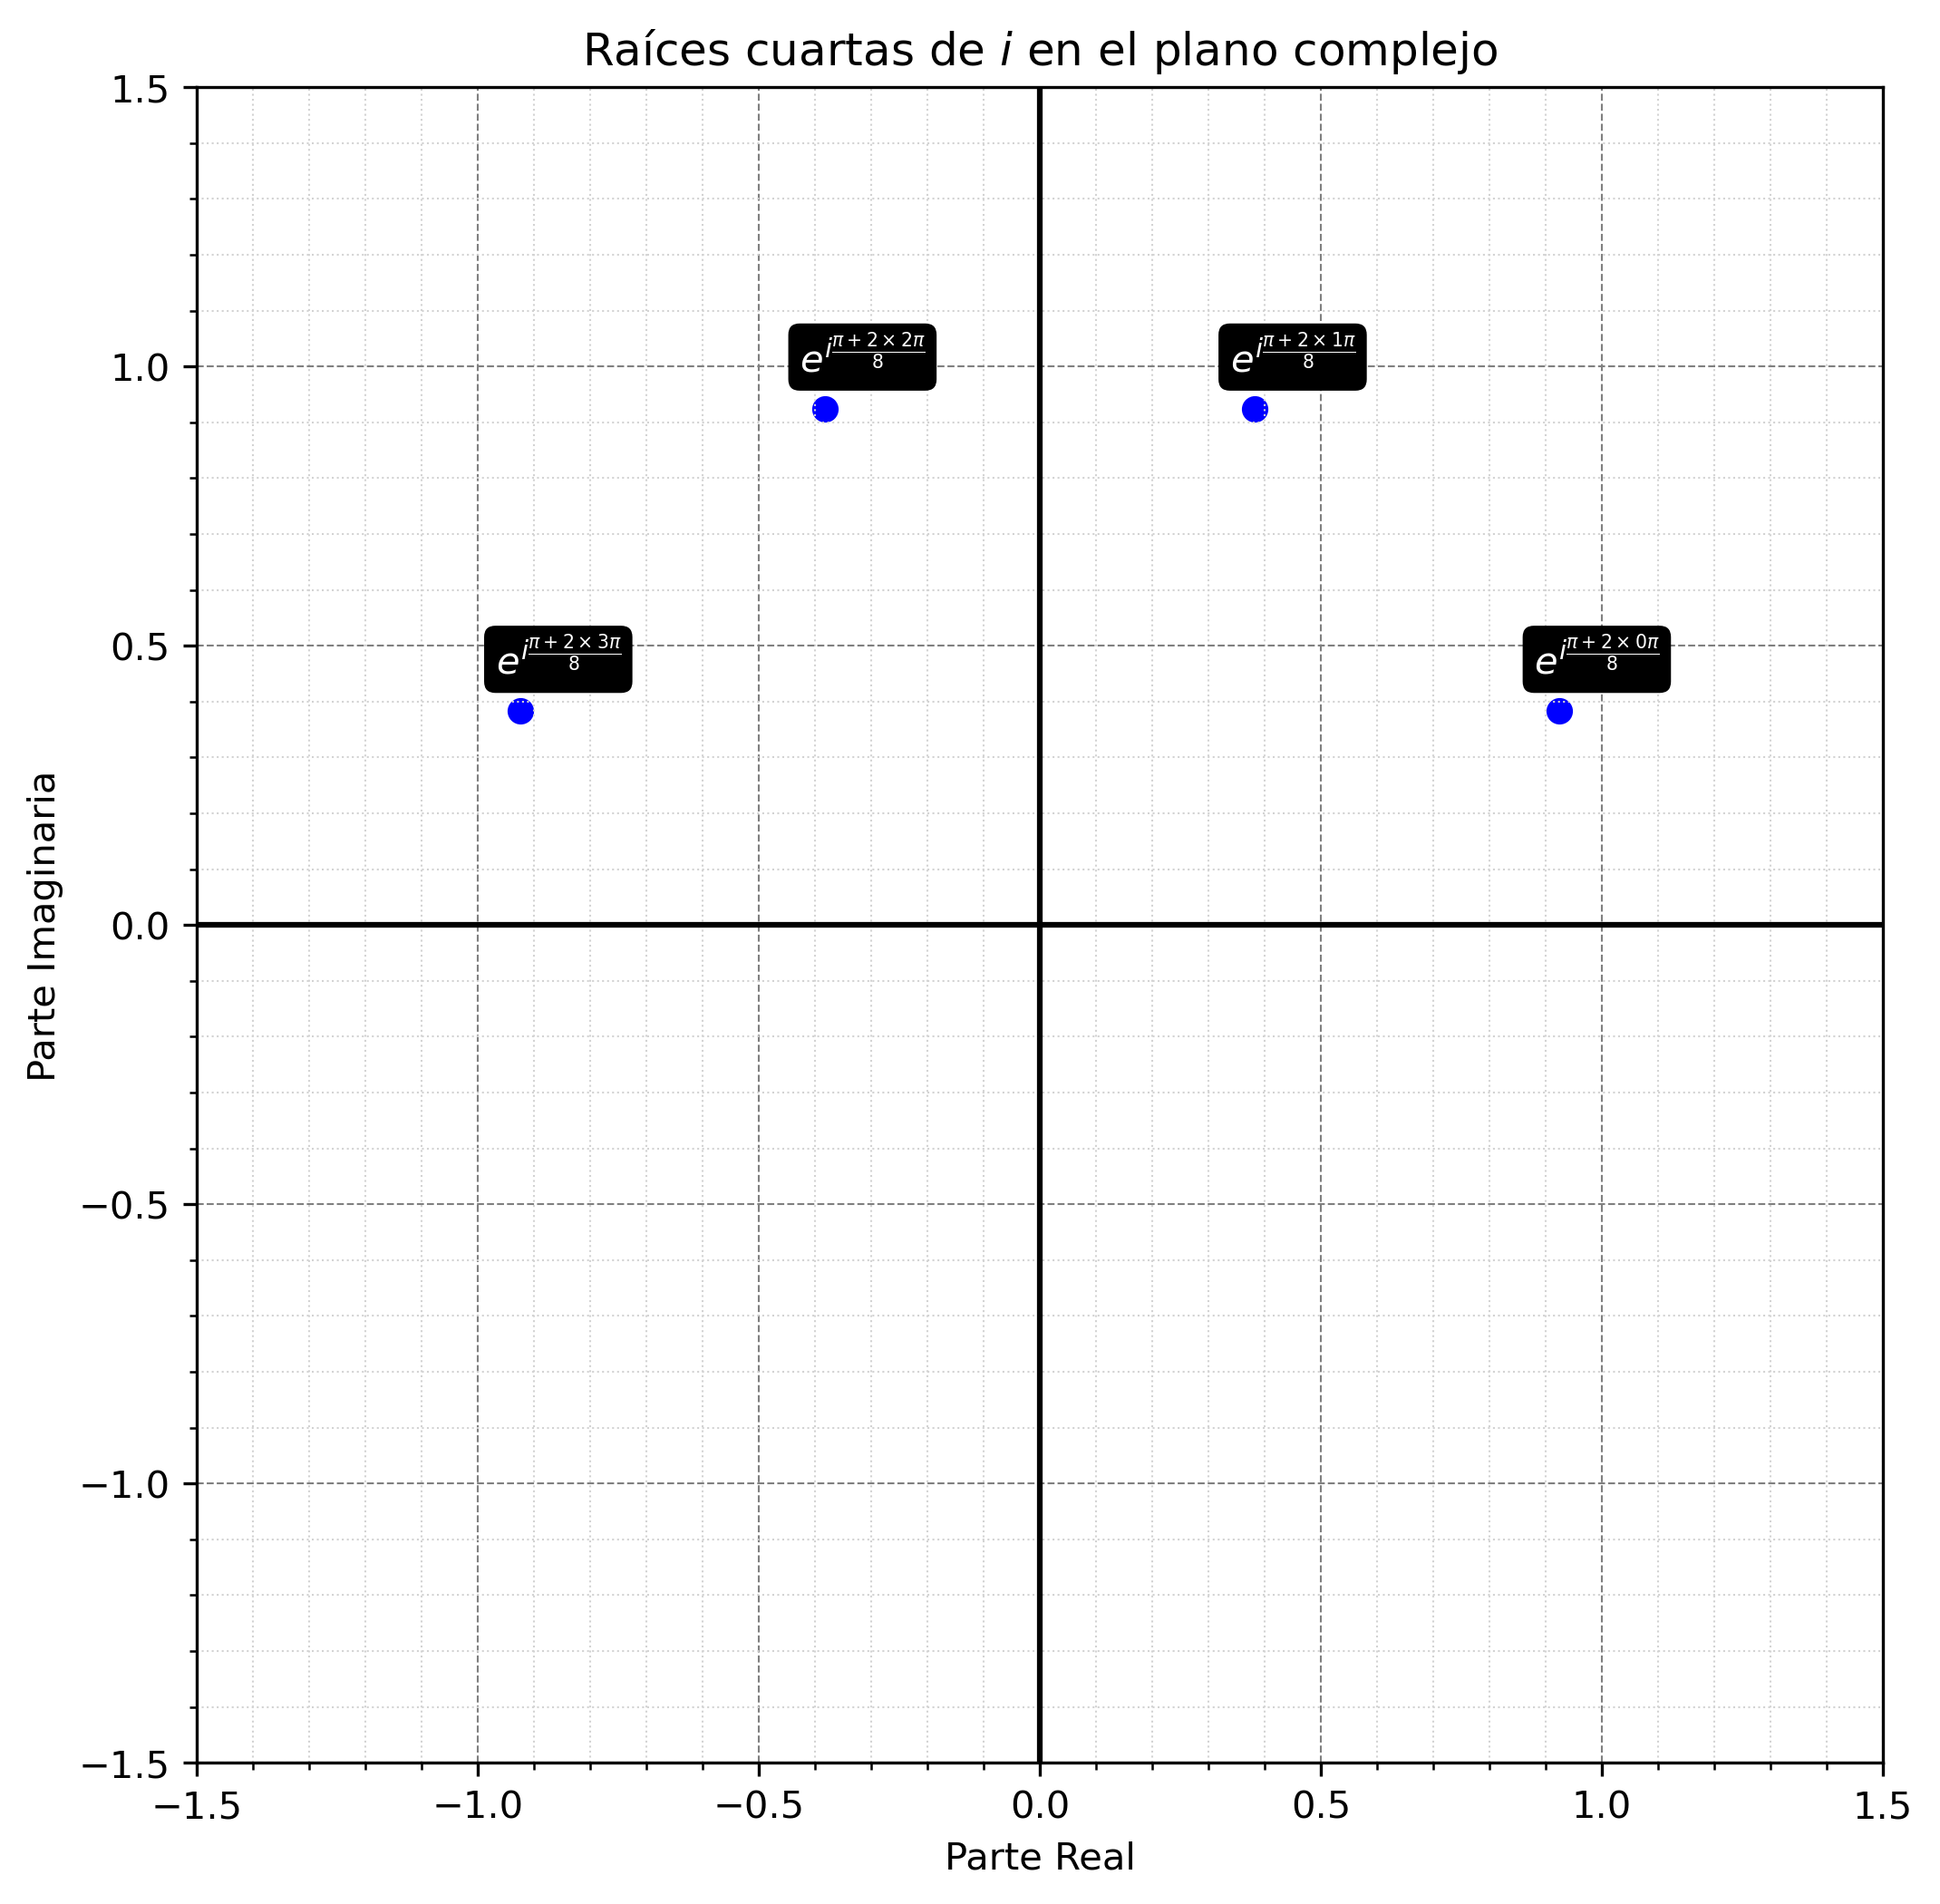
\includegraphics[scale=0.4]{images/grafico_raices_cuartas_i.png}  
        \end{center}
      \item $-16$.\\
        Note que:
        \begin{align*}
          -16=16e^{i\pi}
        \end{align*}
        luego razonando análogamente al punto anterior:
        \begin{align*}
          z&=2e^{i\frac{\pi+2k\pi}{4}} &&\text{Con $k=0,1,2,3$},
        \end{align*}
        por lo que el gráfico se verá de la siguiente forma:
        \begin{center}
          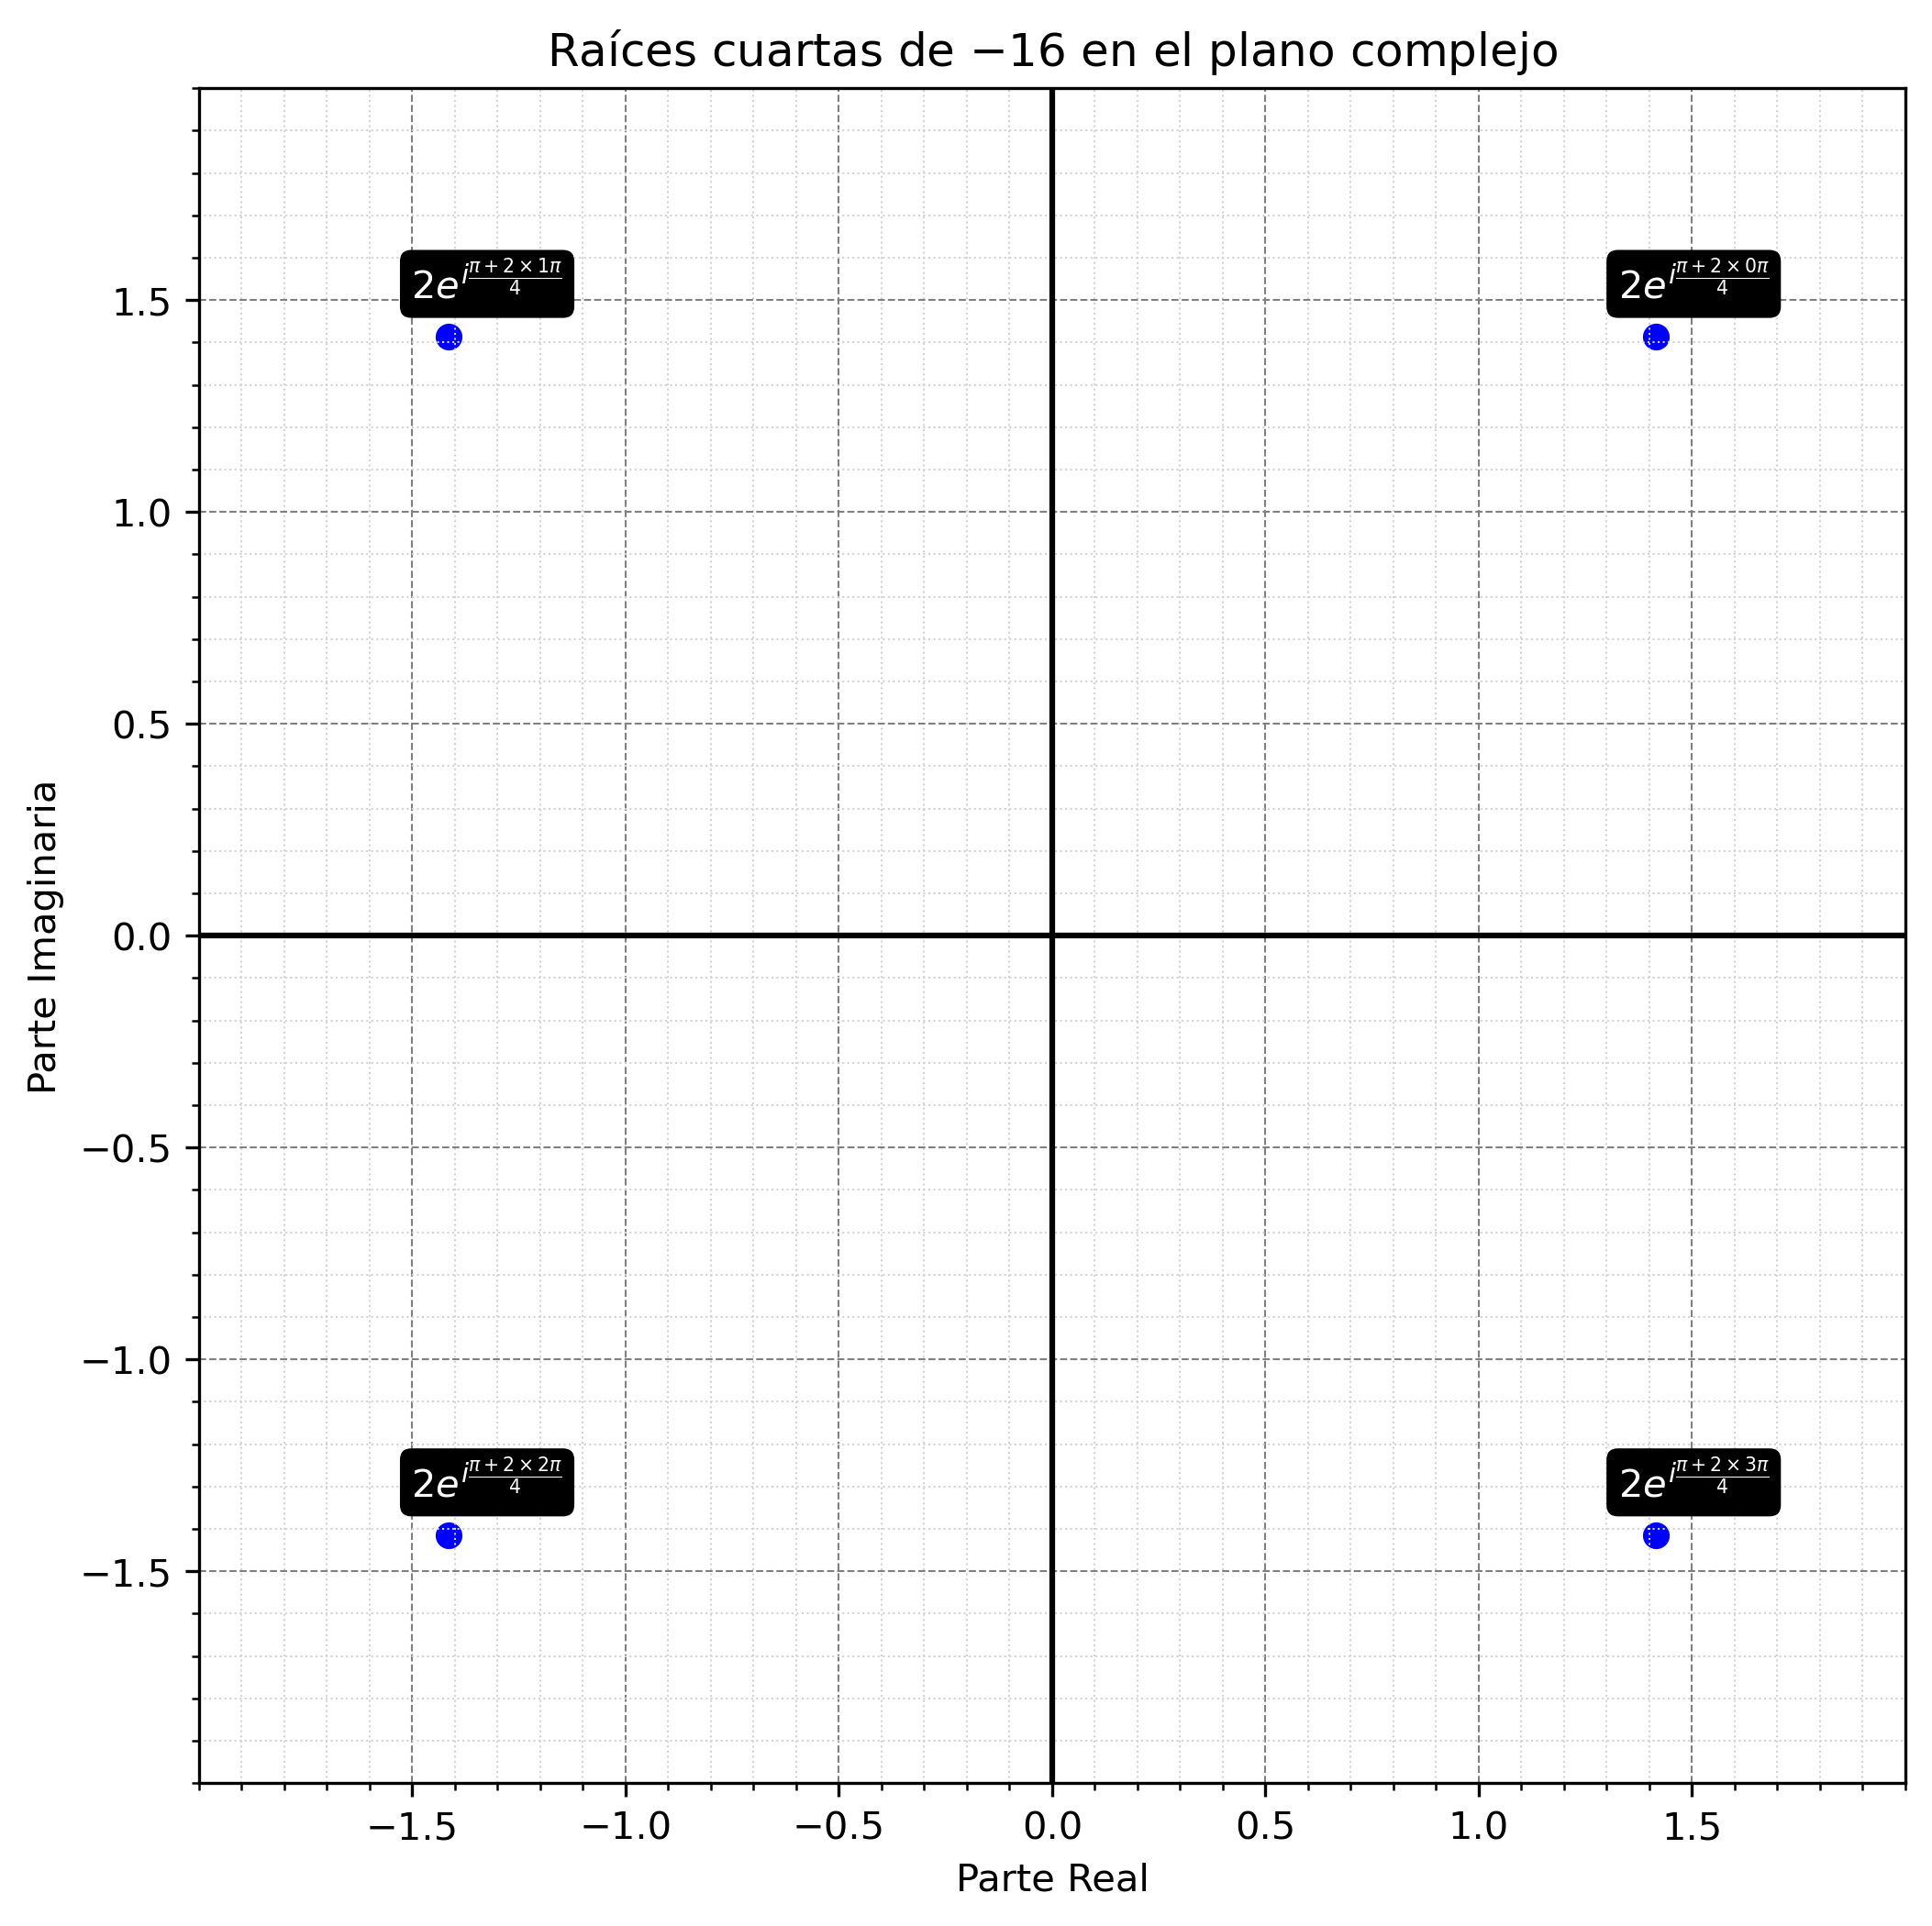
\includegraphics[scale=0.4]{images/grafico_raices_cuartas_-16.png}  
        \end{center}
      \item $-2+2i\sqrt{3}$.\\
        Note que:
        \begin{align*}
          -2+2i\sqrt{3}&=4e^{i\frac{-\pi}{3}},
        \end{align*}
        de forma análoga:
        \begin{align*}
          z&=\sqrt{2}e^{i\frac{-\pi+2k\pi}{6}} &&\text{Con $k=0,1,2,3$},
        \end{align*}
        por lo que el gráfico se verá de la siguiente forma:
        \begin{center}
          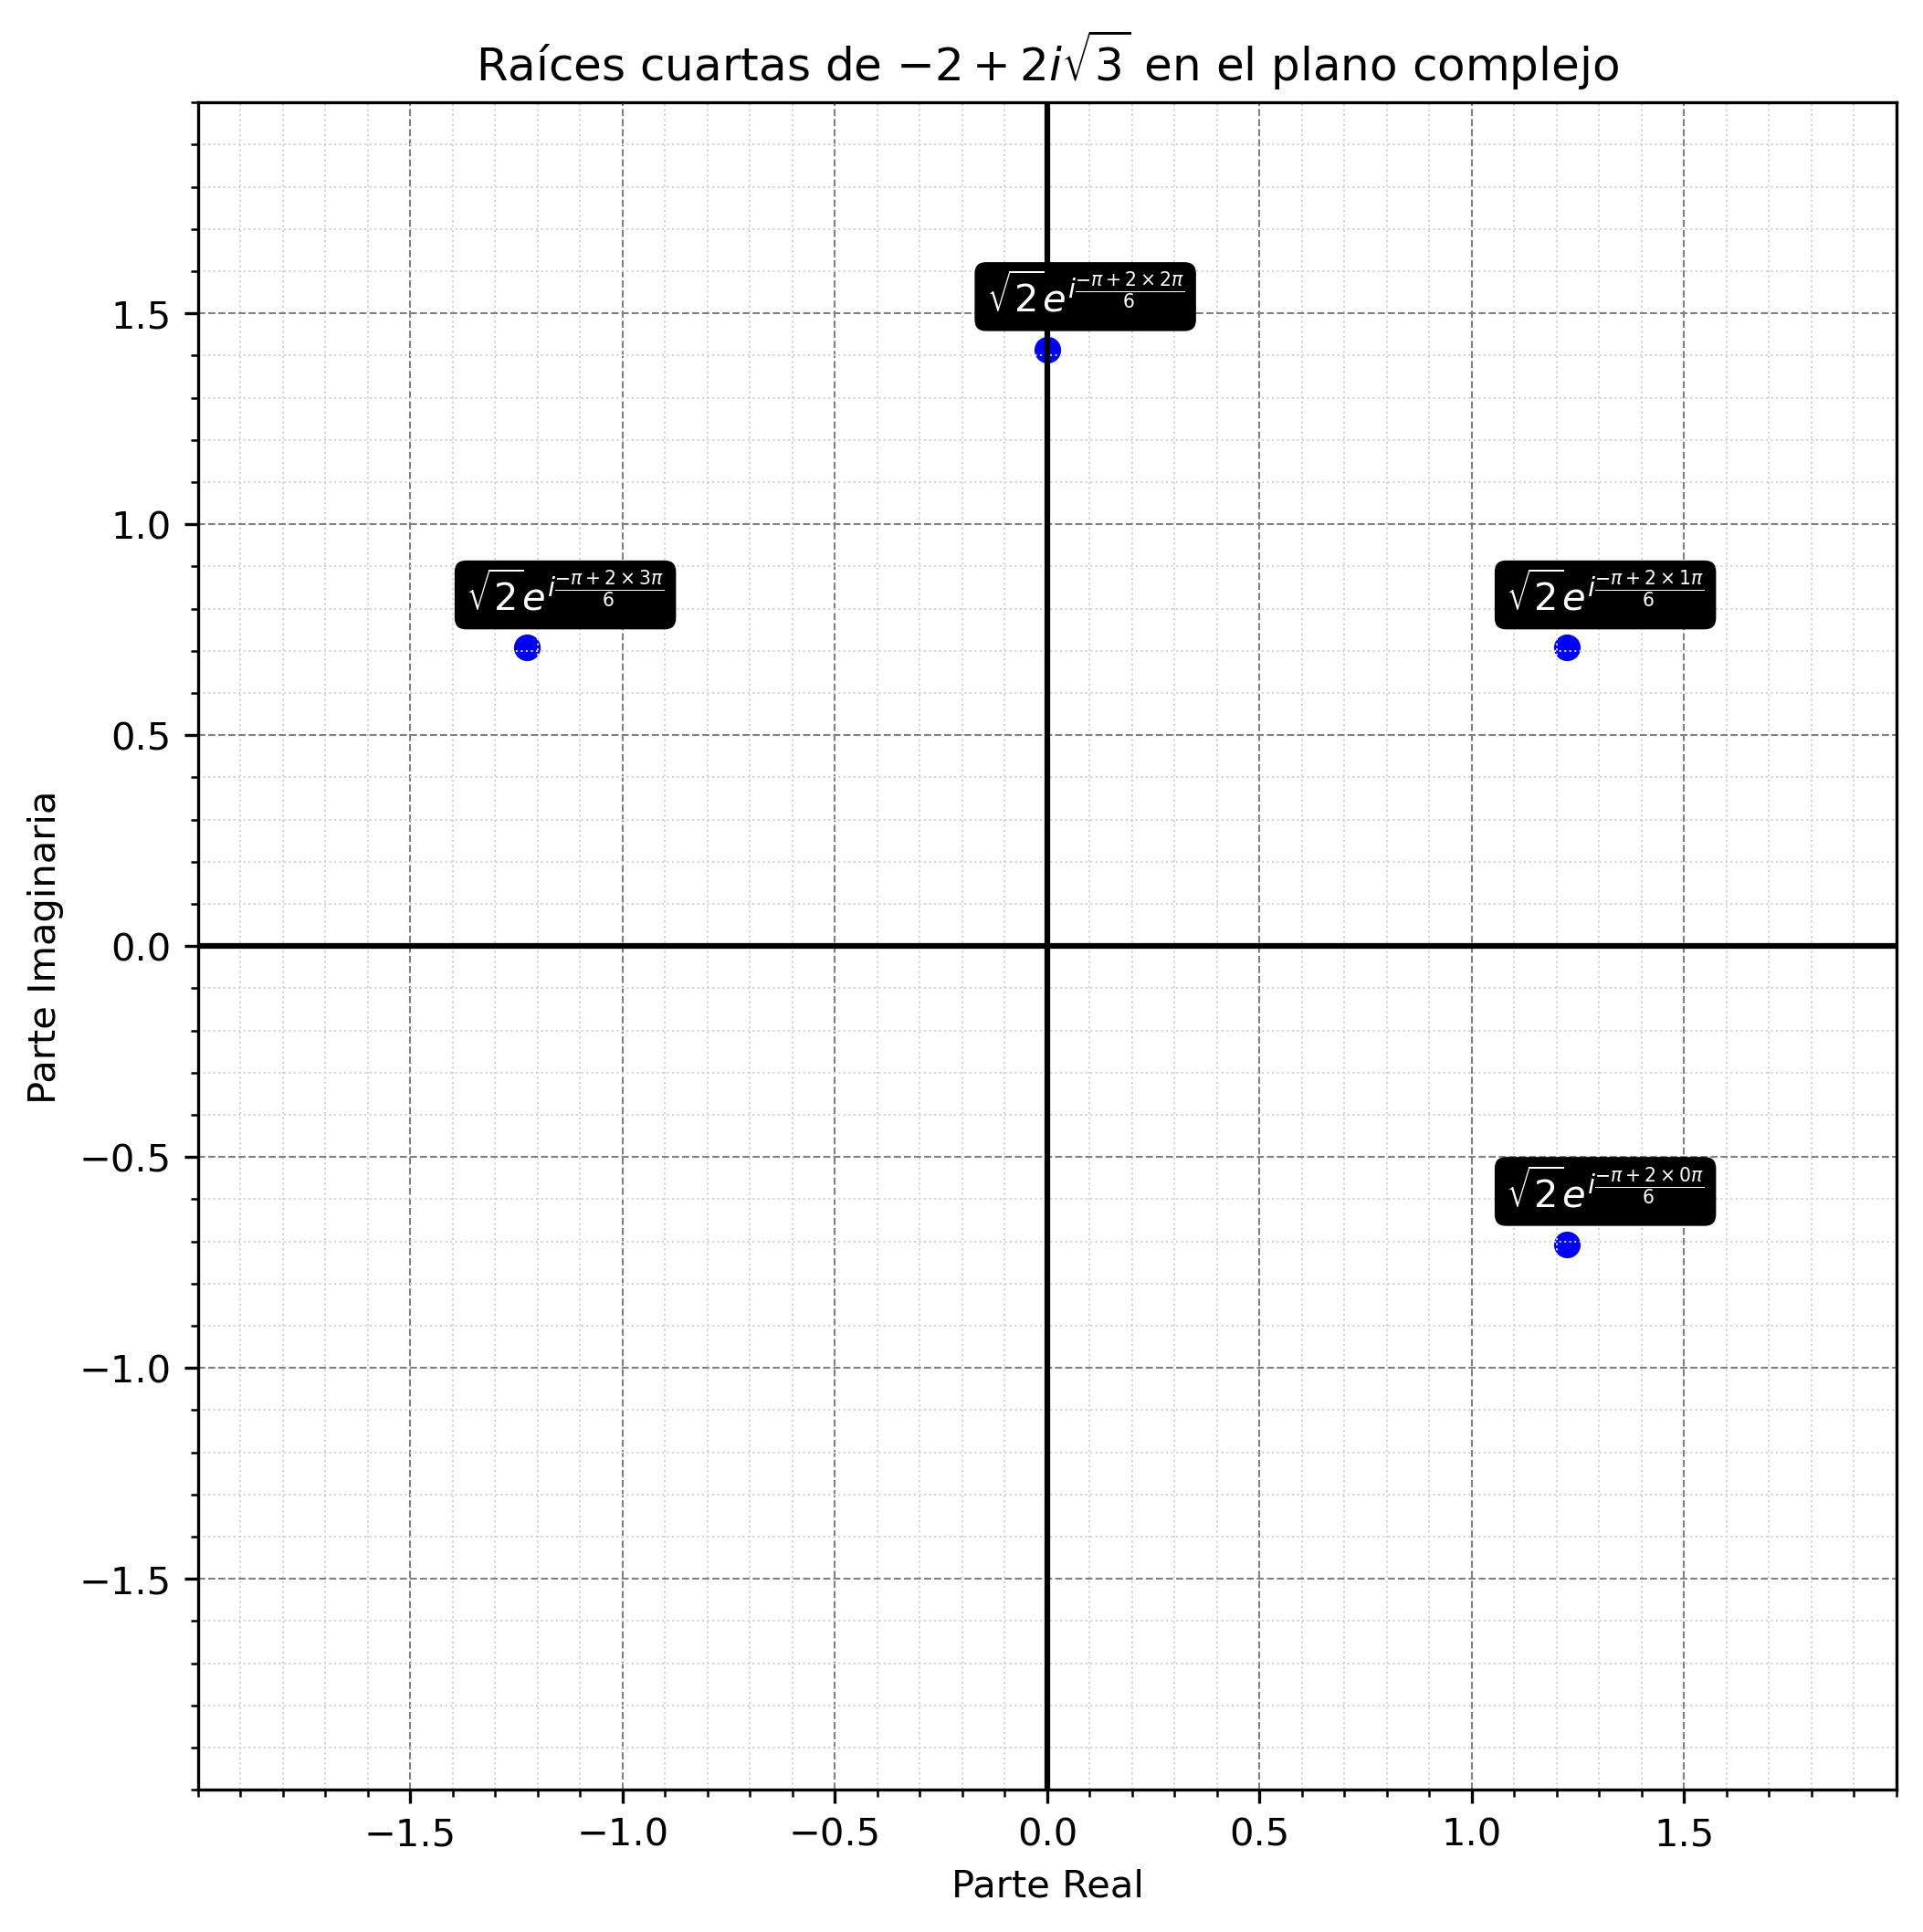
\includegraphics[scale=0.4]{images/grafico_raices_cuartas_-2+2isqrt3.png}  
        \end{center}
    \end{enumerate}
  \end{solution}
\end{homeworkProblem}
